\documentclass[tikz]{standalone}

\def\lecture#1#2#3#4#5#6{
	\node [annotation, #3, scale=0.65, text width=4cm, inner sep=2mm] 
		at (#4) {
		Lecture #1: \textcolor{orange}{\textbf{#2}}
		 \list{--}{\topsep=2pt\itemsep=0pt\parsep=0pt
		 \parskip=0pt\labelwidth=8pt\leftmargin=8pt
		 \itemindent=0pt\labelsep=2pt}
		 #5
		 \endlist
		 v
		 BOO
	};
}

\usetikzlibrary{mindmap,trees,backgrounds, shadows}

\begin{document}
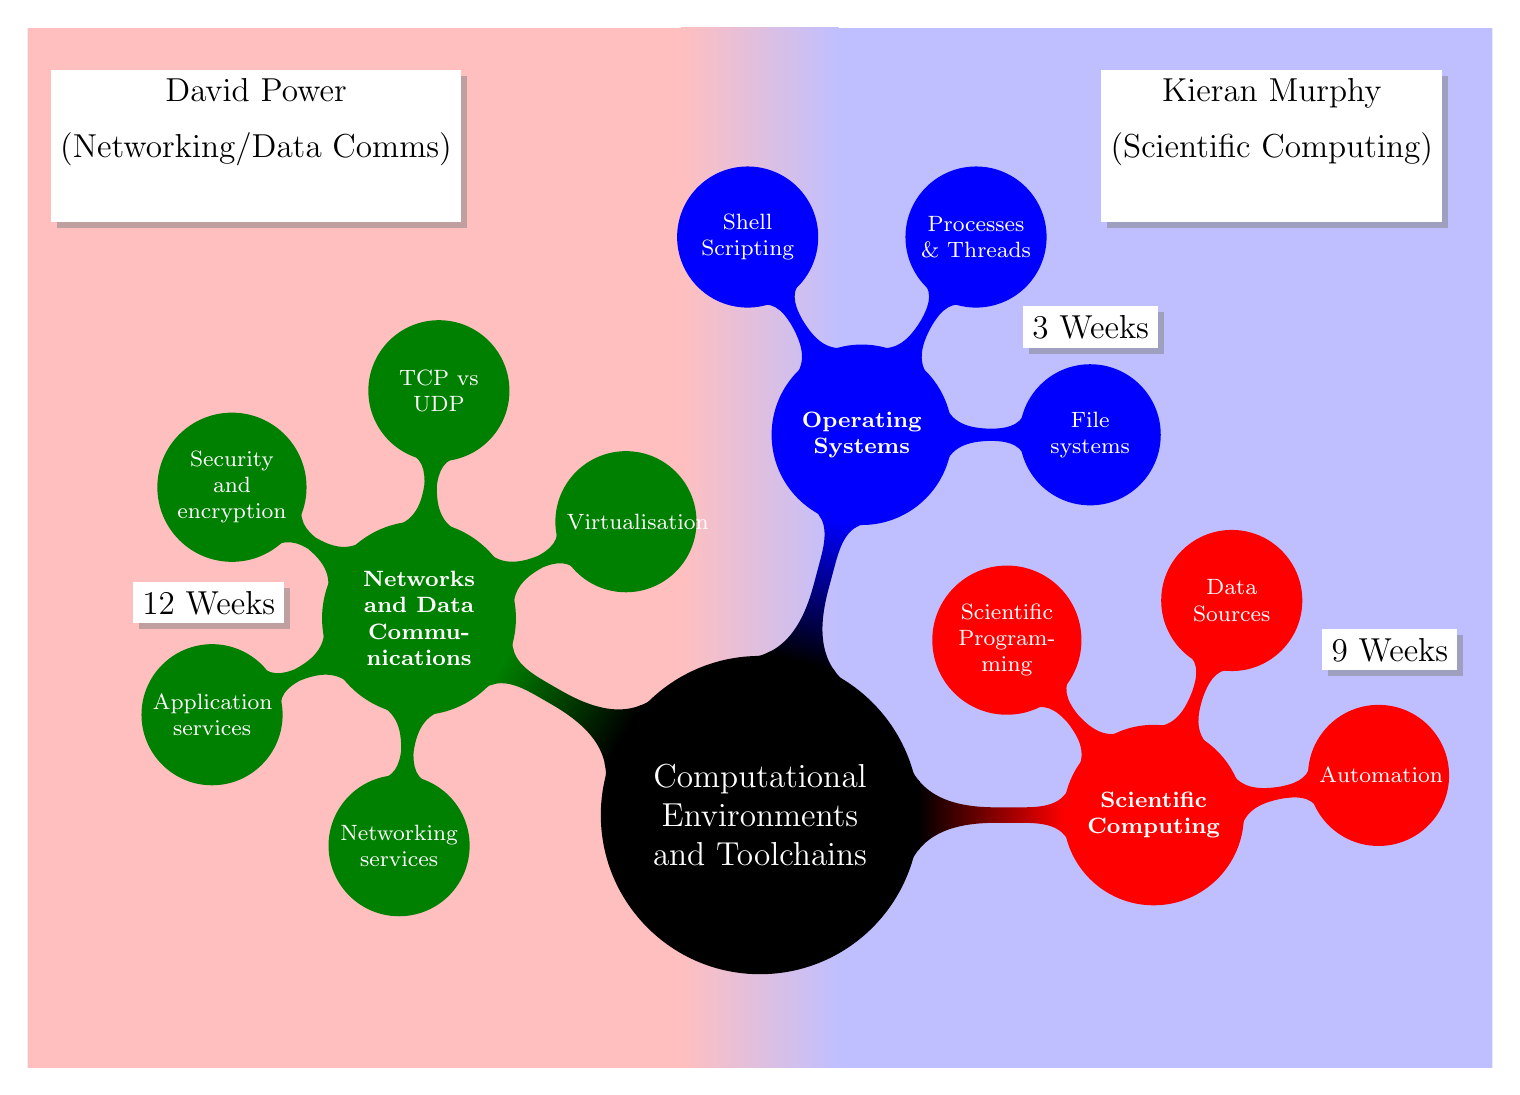
\begin{tikzpicture}
	\path[mindmap,concept color=black,text=white,
	root concept/.append style={
		concept,
		circular drop shadow, fill=white, line width=1ex, 
		text=black, font=\large\scshape},
	level 1 concept/.append style =
      {font=\footnotesize\bfseries, sibling angle=75},
      ]
		node[concept] (M) {Computational Environments and Toolchains}
			[clockwise from=150,rectangle]
			child[concept color=green!50!black] {
				node[concept] {Networks and Data Communications}
					[clockwise from=-95]
					child { node[concept] {Networking services} }
					child { node[concept] {Application services} }
					child { node[concept] {Security and encryption} }
					child { node[concept] {TCP vs UDP} }
					child { node[concept] {Virtualisation} }
			}  
			child[concept color=blue] {
				node[concept] {Operating Systems}
					[clockwise from=120]
					child { node[concept] {Shell Scripting} }
					%child { node[concept] {Virtualisation} }
					child { node[concept] {Processes \& Threads} }
					%child { node[concept] {Parallel Programming} }
					child { node[concept] {File systems} }
			}
			child[concept color=red] { 
				node[concept]  {Scientific Computing}
					[clockwise from=130] 
					child { node[concept] (Programming) {Scientific Programming} }
					child { node[concept] {Data Sources} }
					%child { node[concept] {Document Generation} }
					child { node[concept] {Automation} }
					%child { node[concept] {Publication} }
			}
    ;
    
%\lecture{1}{Comp}{above}{Programming}{\item Pyhon}{df}

	\begin{pgfonlayer}{background}
	    \clip (-9.3,-3.2) rectangle (9.3,10);
	    \colorlet{upperleft}{red!25}
	    \colorlet{upperright}{blue!25}
	    \colorlet{lowerleft}{red!25}
	    \colorlet{lowerright}{blue!25}
	    \fill [lowerleft] (M) rectangle ++(-10,10);
	    \fill [lowerleft] (M) rectangle ++(-10,-5);
	    \fill [lowerright] (M) rectangle ++(10,10);
	    \fill [lowerright] (M) rectangle ++(10,-5);
	    % The shadings:
		\shade [left color=upperleft,right color=upperright] (M) 
		(-1,-5) rectangle ++(2,15);
	  \end{pgfonlayer}
	
	\tikzstyle{lecturer}=[drop shadow,fill=white,font=\large]
	\node[lecturer,align=center] at (-6.4,8.5) {David Power\\[6pt]
		(Networking/Data Comms)\\[6pt]
		};
	\node[lecturer,align=center] at (6.5,8.5) {Kieran Murphy\\[6pt]
	(Scientific Computing)\\[6pt]
	};
	
	\node[lecturer] at (-7,2.7) {12 Weeks};
	\node[lecturer] at (8,2.1) {9 Weeks};
	\node[lecturer] at (4.2,6.2) {3 Weeks};
\end{tikzpicture}

\end{document}